\chapter{Results}
\label{c:results}
In diesem Kapitel sollest du den Vergleich deiner Implementation mit den bestehenden Apps machen und deine Arbeit zusammenfassen.

\todo{RENAME THE APPS FROM MASWE\_... TO MASVS\_...}

We developed three separate apps, which are named \texttt{maswe\_storage}, \texttt{maswe\_crypto}, and \texttt{maswe\_platform}. They contain a total of 28 vulnerabilities, covering all six vulnerabilities described by MASVS-STORAGE and all 18 MASVS-CRYPTO vulnerabilities. The remaining four implemented vulnerabilities are part of MASVS-PLATFORM. This means we created implementations for 28 out of 115 vulnerabilities documented by OWASP MASWE, covering about 25\% of the entire vulnerability catalog. Each vulnerability has its own documentation, explaining where it can be found in the code and how it can be exploited. Depending on the vulnerability, the documentation also includes links to interesting and relevant articles and tools related to the vulnerability and sometimes describes  how the vulnerability can be fixed. All implemented vulnerabilities are mapped and linked to their respective OWASP MASWE counterpart.

The code for our apps is entirely open source and available on GitHub \todo{Add source+reference to my GitHub repo here}. It contains a checklist \todo{add ref to the checklist} of all vulnerabilities as described by OWASP MASWE, which gives an overview for which vulnerabilities are implemented, which are being worked on, and which are thus far not worked on. Every vulnerability in this overview has an indicator of its status in OWASP MASWE, showing whether the vulnerability is still in beta and lacks proper documentation by OWASP, is fully detailed, or already being considered deprecated and should not to be considered anymore. This benefits people using the apps and the GitHub repository for educational purposes by allowing them to better see the complete picture of the OWASP vulnerability landscape. It further helps developers aiming to contribute to this project, as it points them to which vulnerabilities are yet to be worked on, and which should be ignored. To further enable future work on this project, the repository is complete with documentation on how developers can contribute, what the expected coding styles are, and what templates should be used for commiting to the project. This enforces a clean and uniform coding style across the project, which further improves its usefulness as an educational tool by not confusing people aiming to learn security principles or penetration testing through confusing and inconsistent code.

For the documentation and the vulnerabilities themselves to stay relevant and for the apps as a whole to be a valid reference resource for the OWASP MASTG, constant maintenance and updating of the Android project is necessary. Without it, our apps develop the same issues as some of the existing MASTG reference apps of becoming outdated and not accurately reflecting the standard set by the OWASP MAS project anymore.

% Struktur
\section{Comparison with Existing Intentionally Vulnerable Android Applications}

\begin{figure}[htbp]
  \centering
  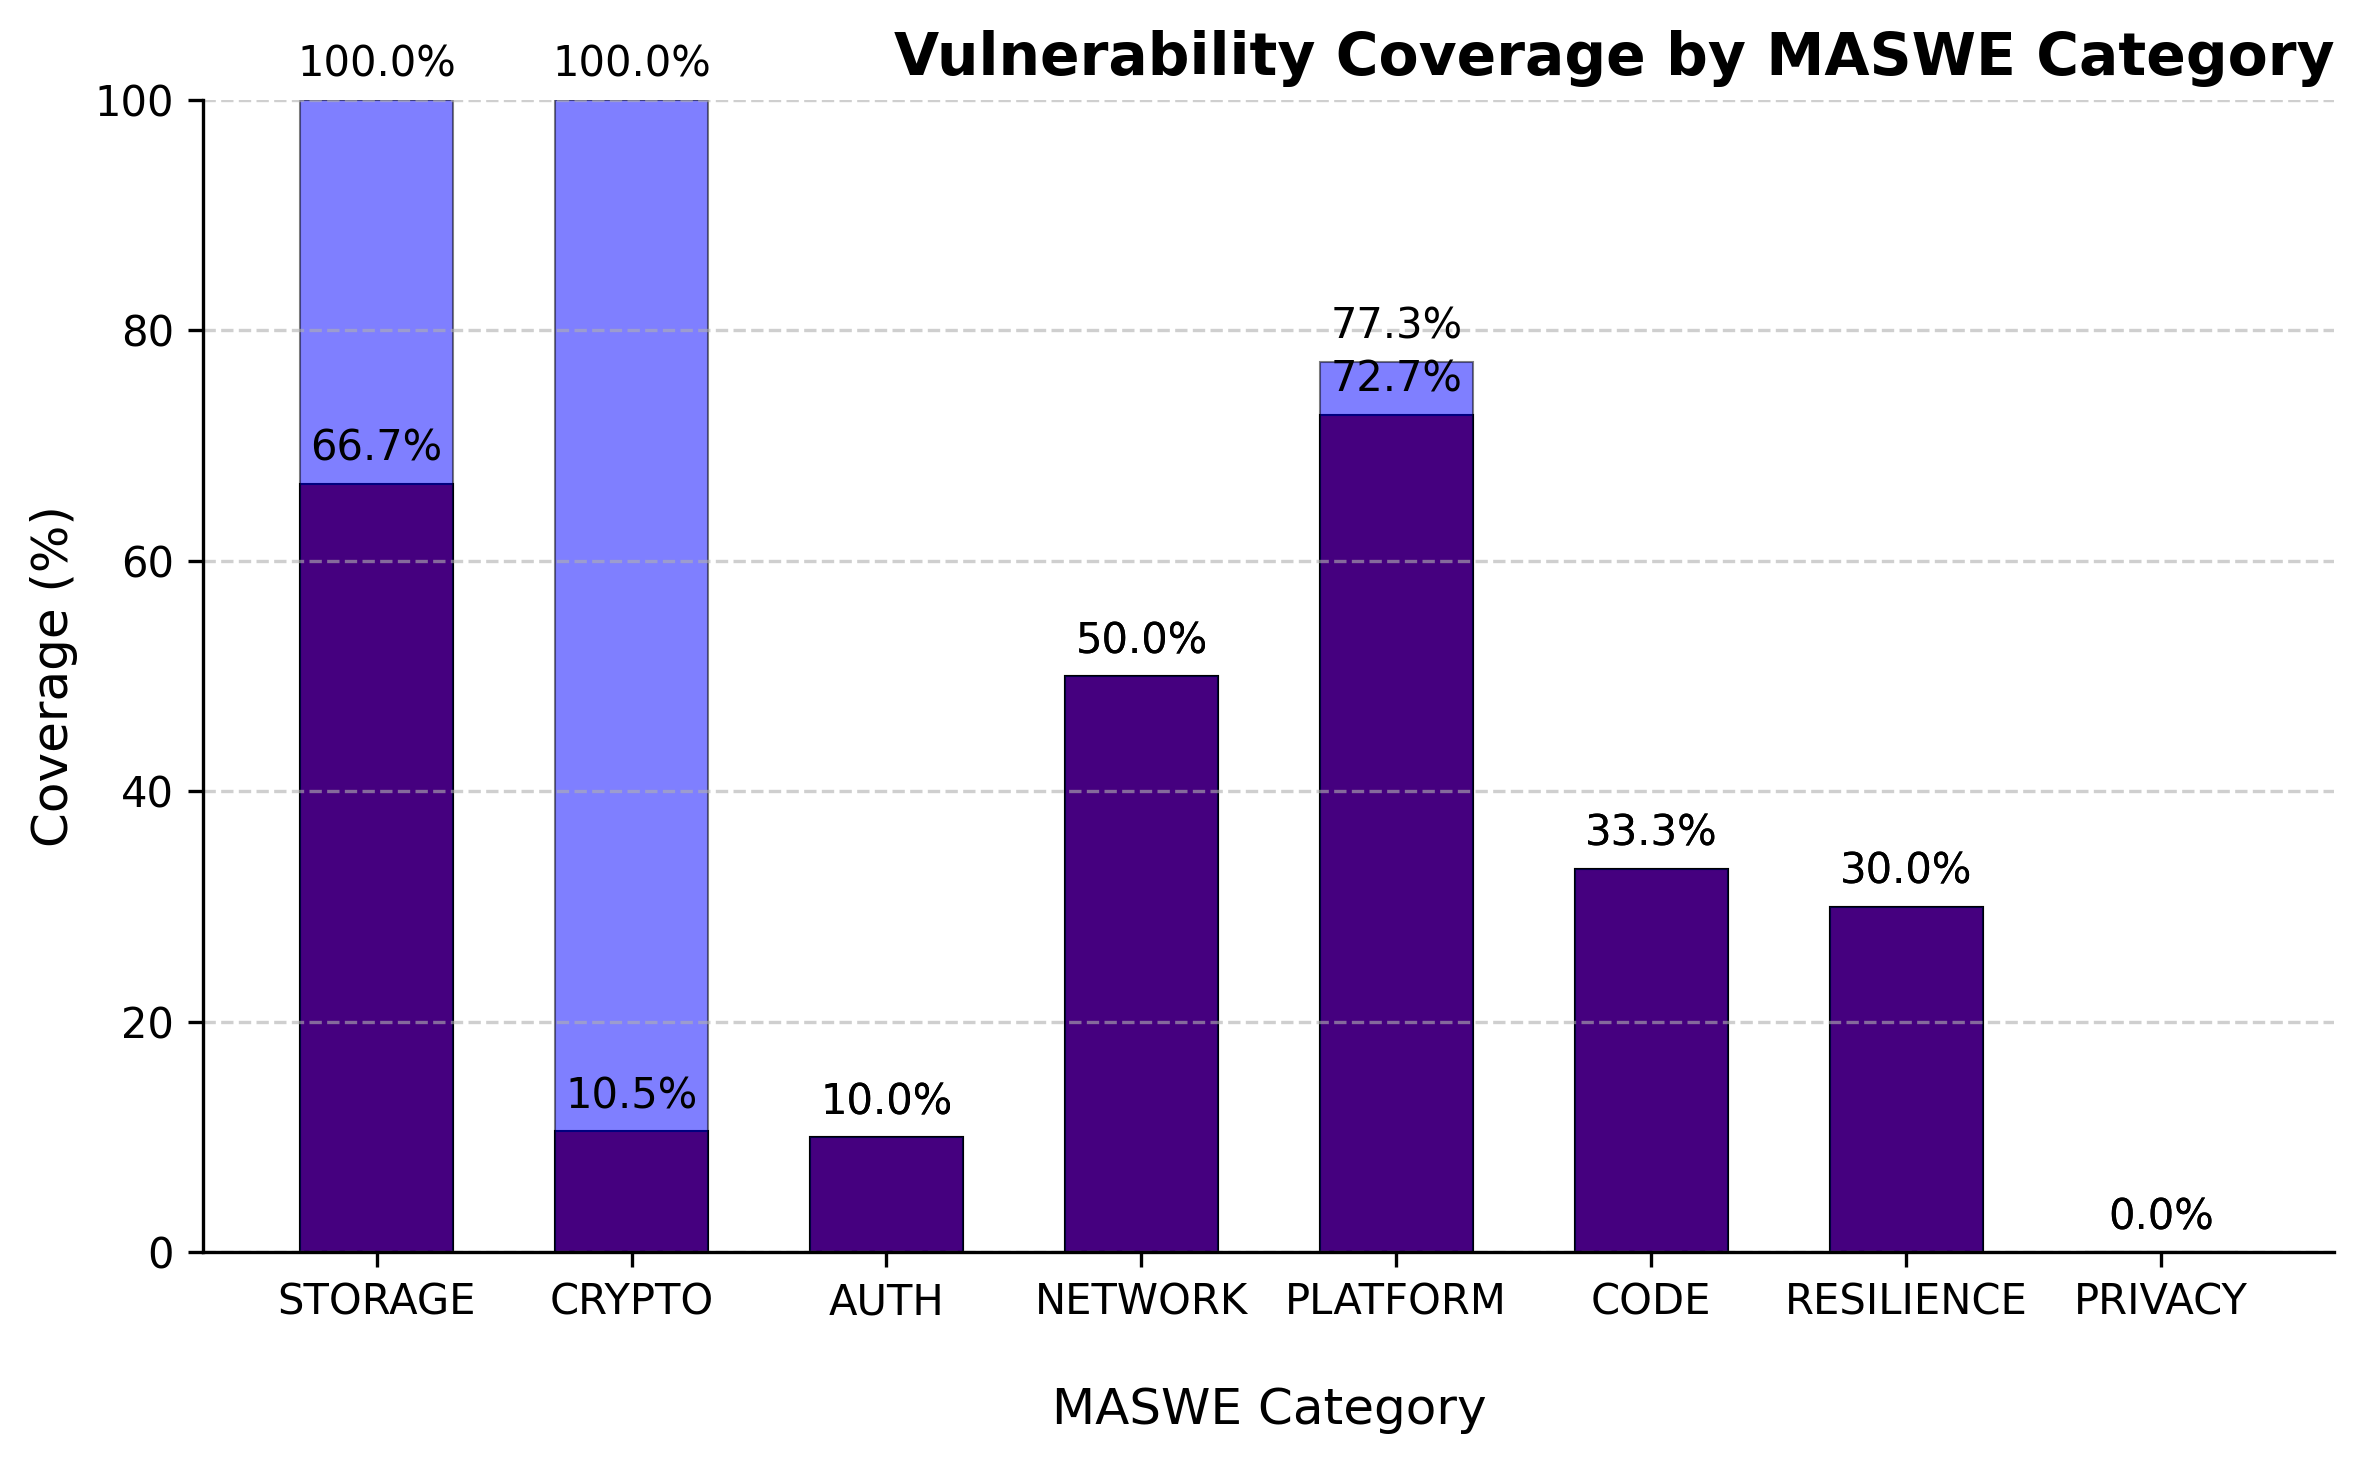
\includegraphics[width=1.0\textwidth]{dev_documents/BA_Thesis_Kronig/figures/results/vulnerability_coverage_percentage_comparison.png}
  \caption{ \todo{Add image caption} }
  \label{fig:}
\end{figure}

\begin{figure}[htbp]
  \centering
  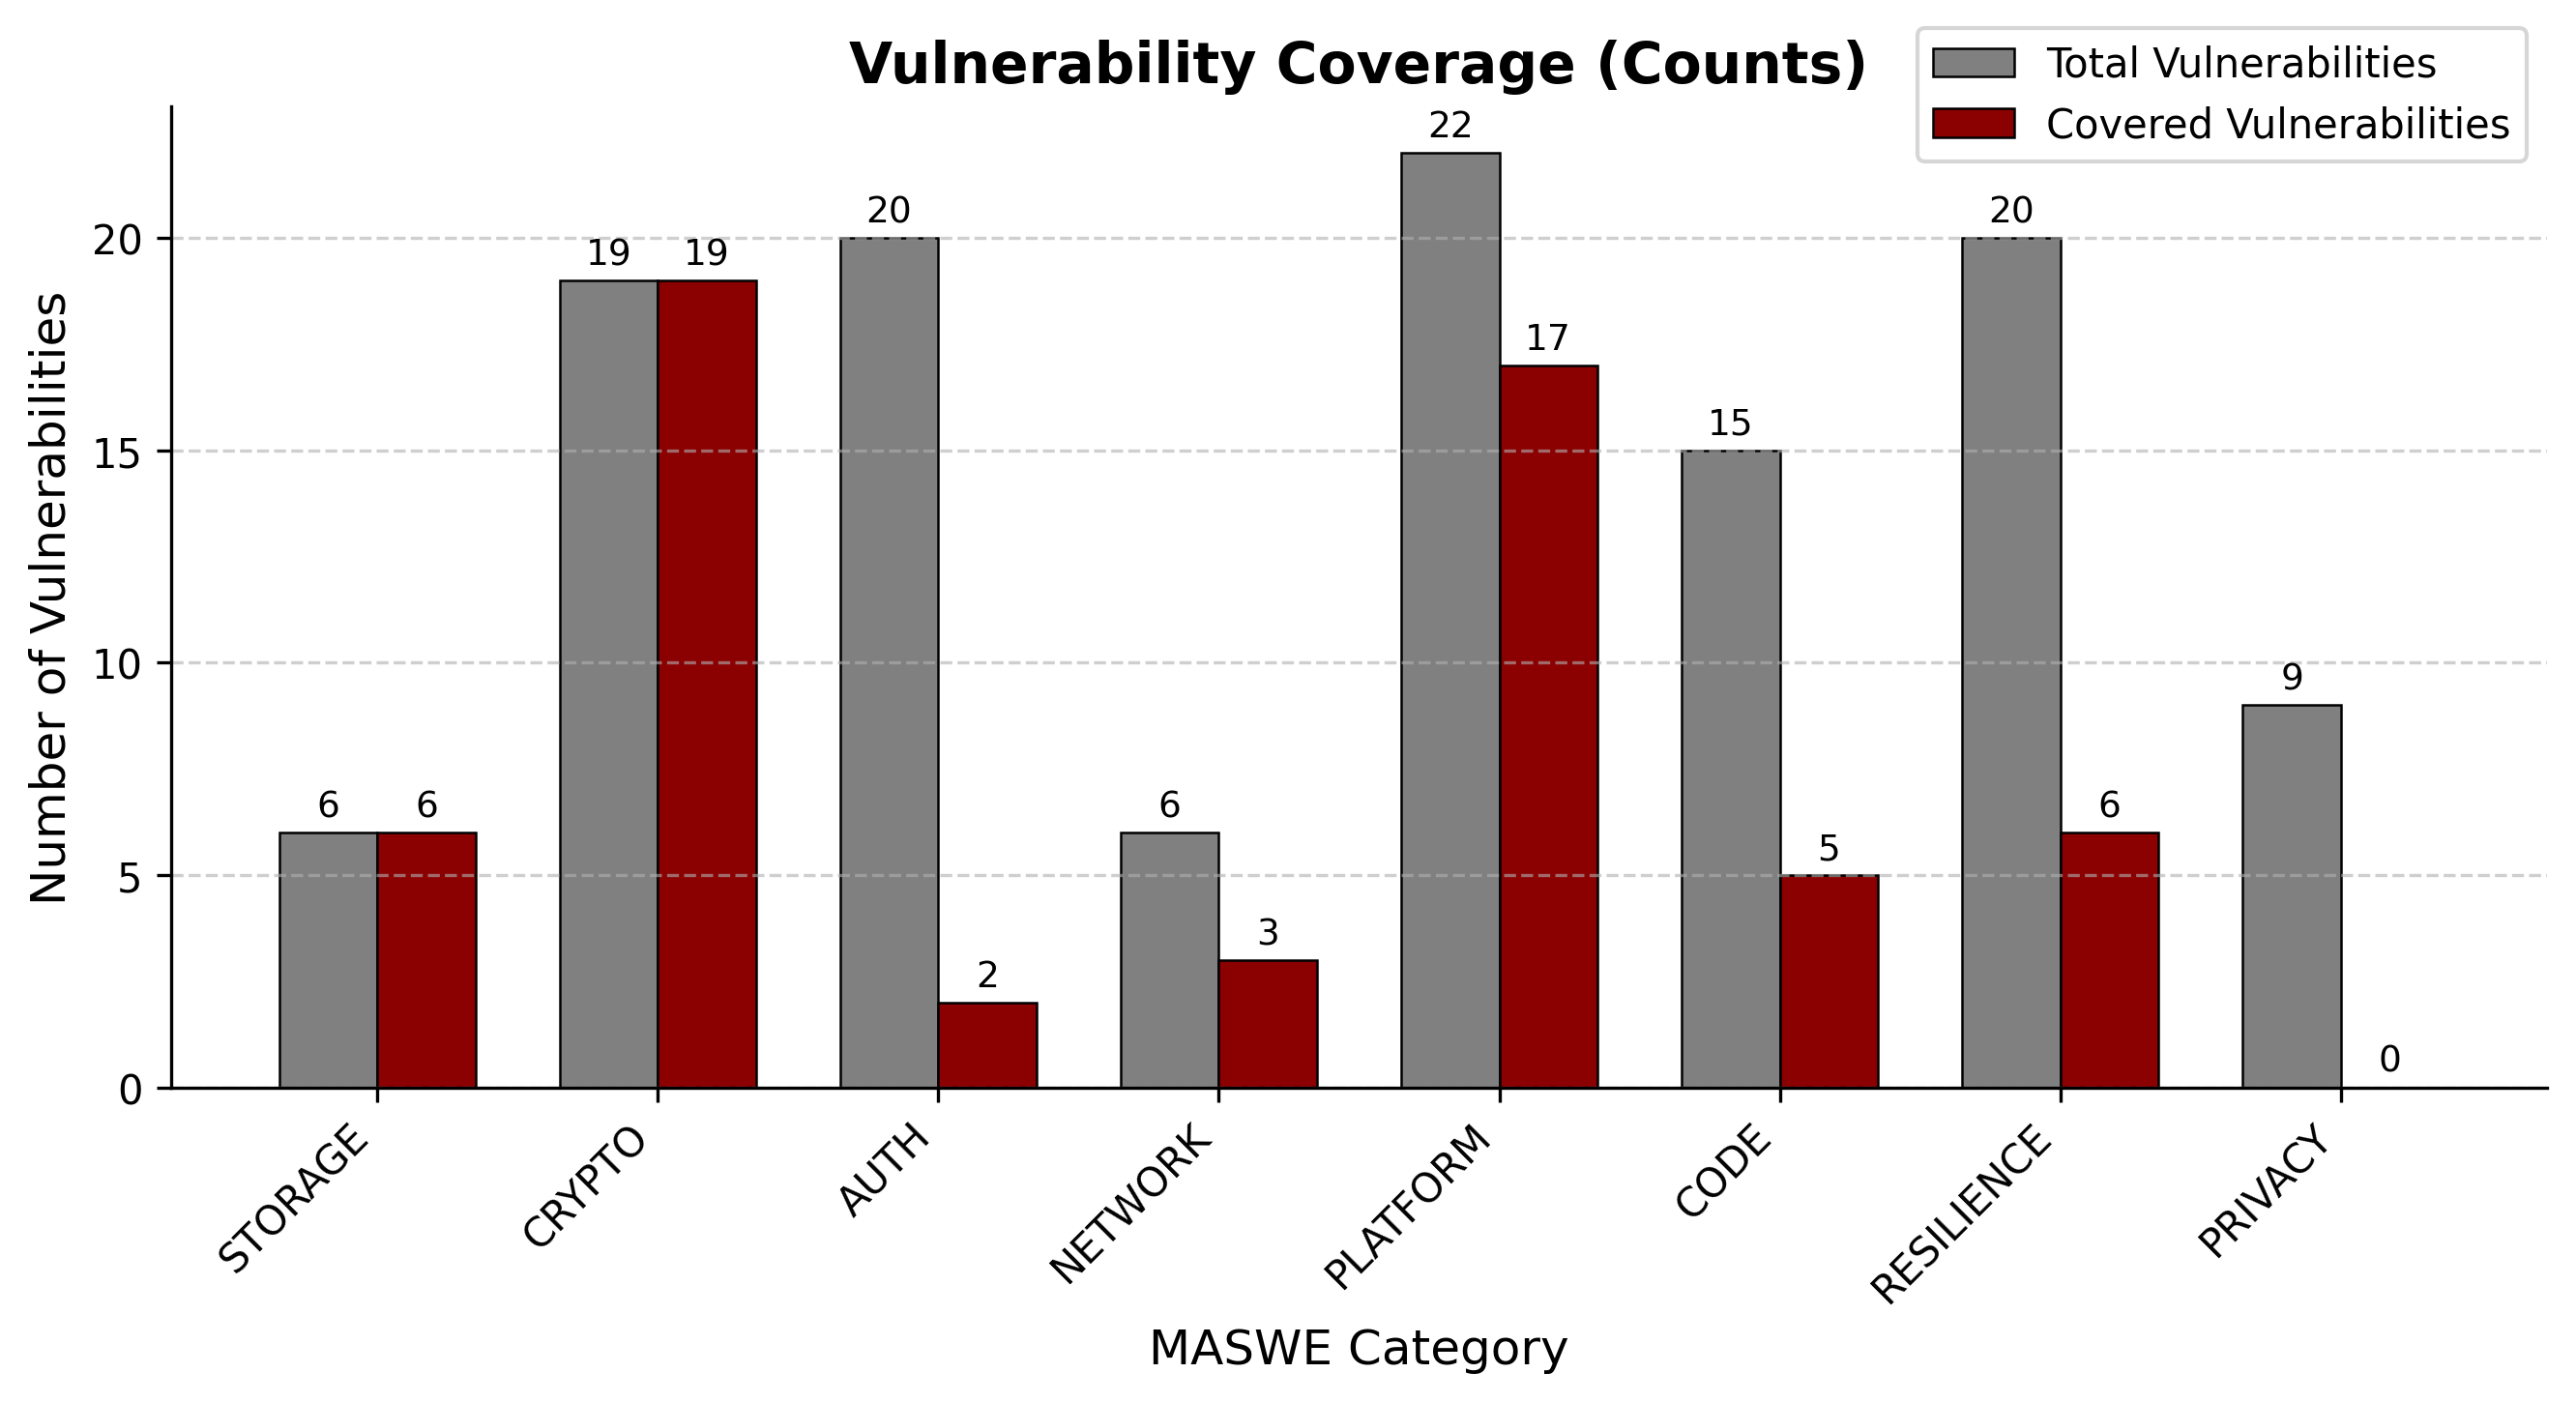
\includegraphics[width=1.0\textwidth]{dev_documents/BA_Thesis_Kronig/figures/results/total_vs_implemented_vulnerability_counts_with_own_app.png}
  \caption{ \todo{Add image caption} }
  \label{fig:}
\end{figure}

\begin{figure}[htbp]
  \centering
  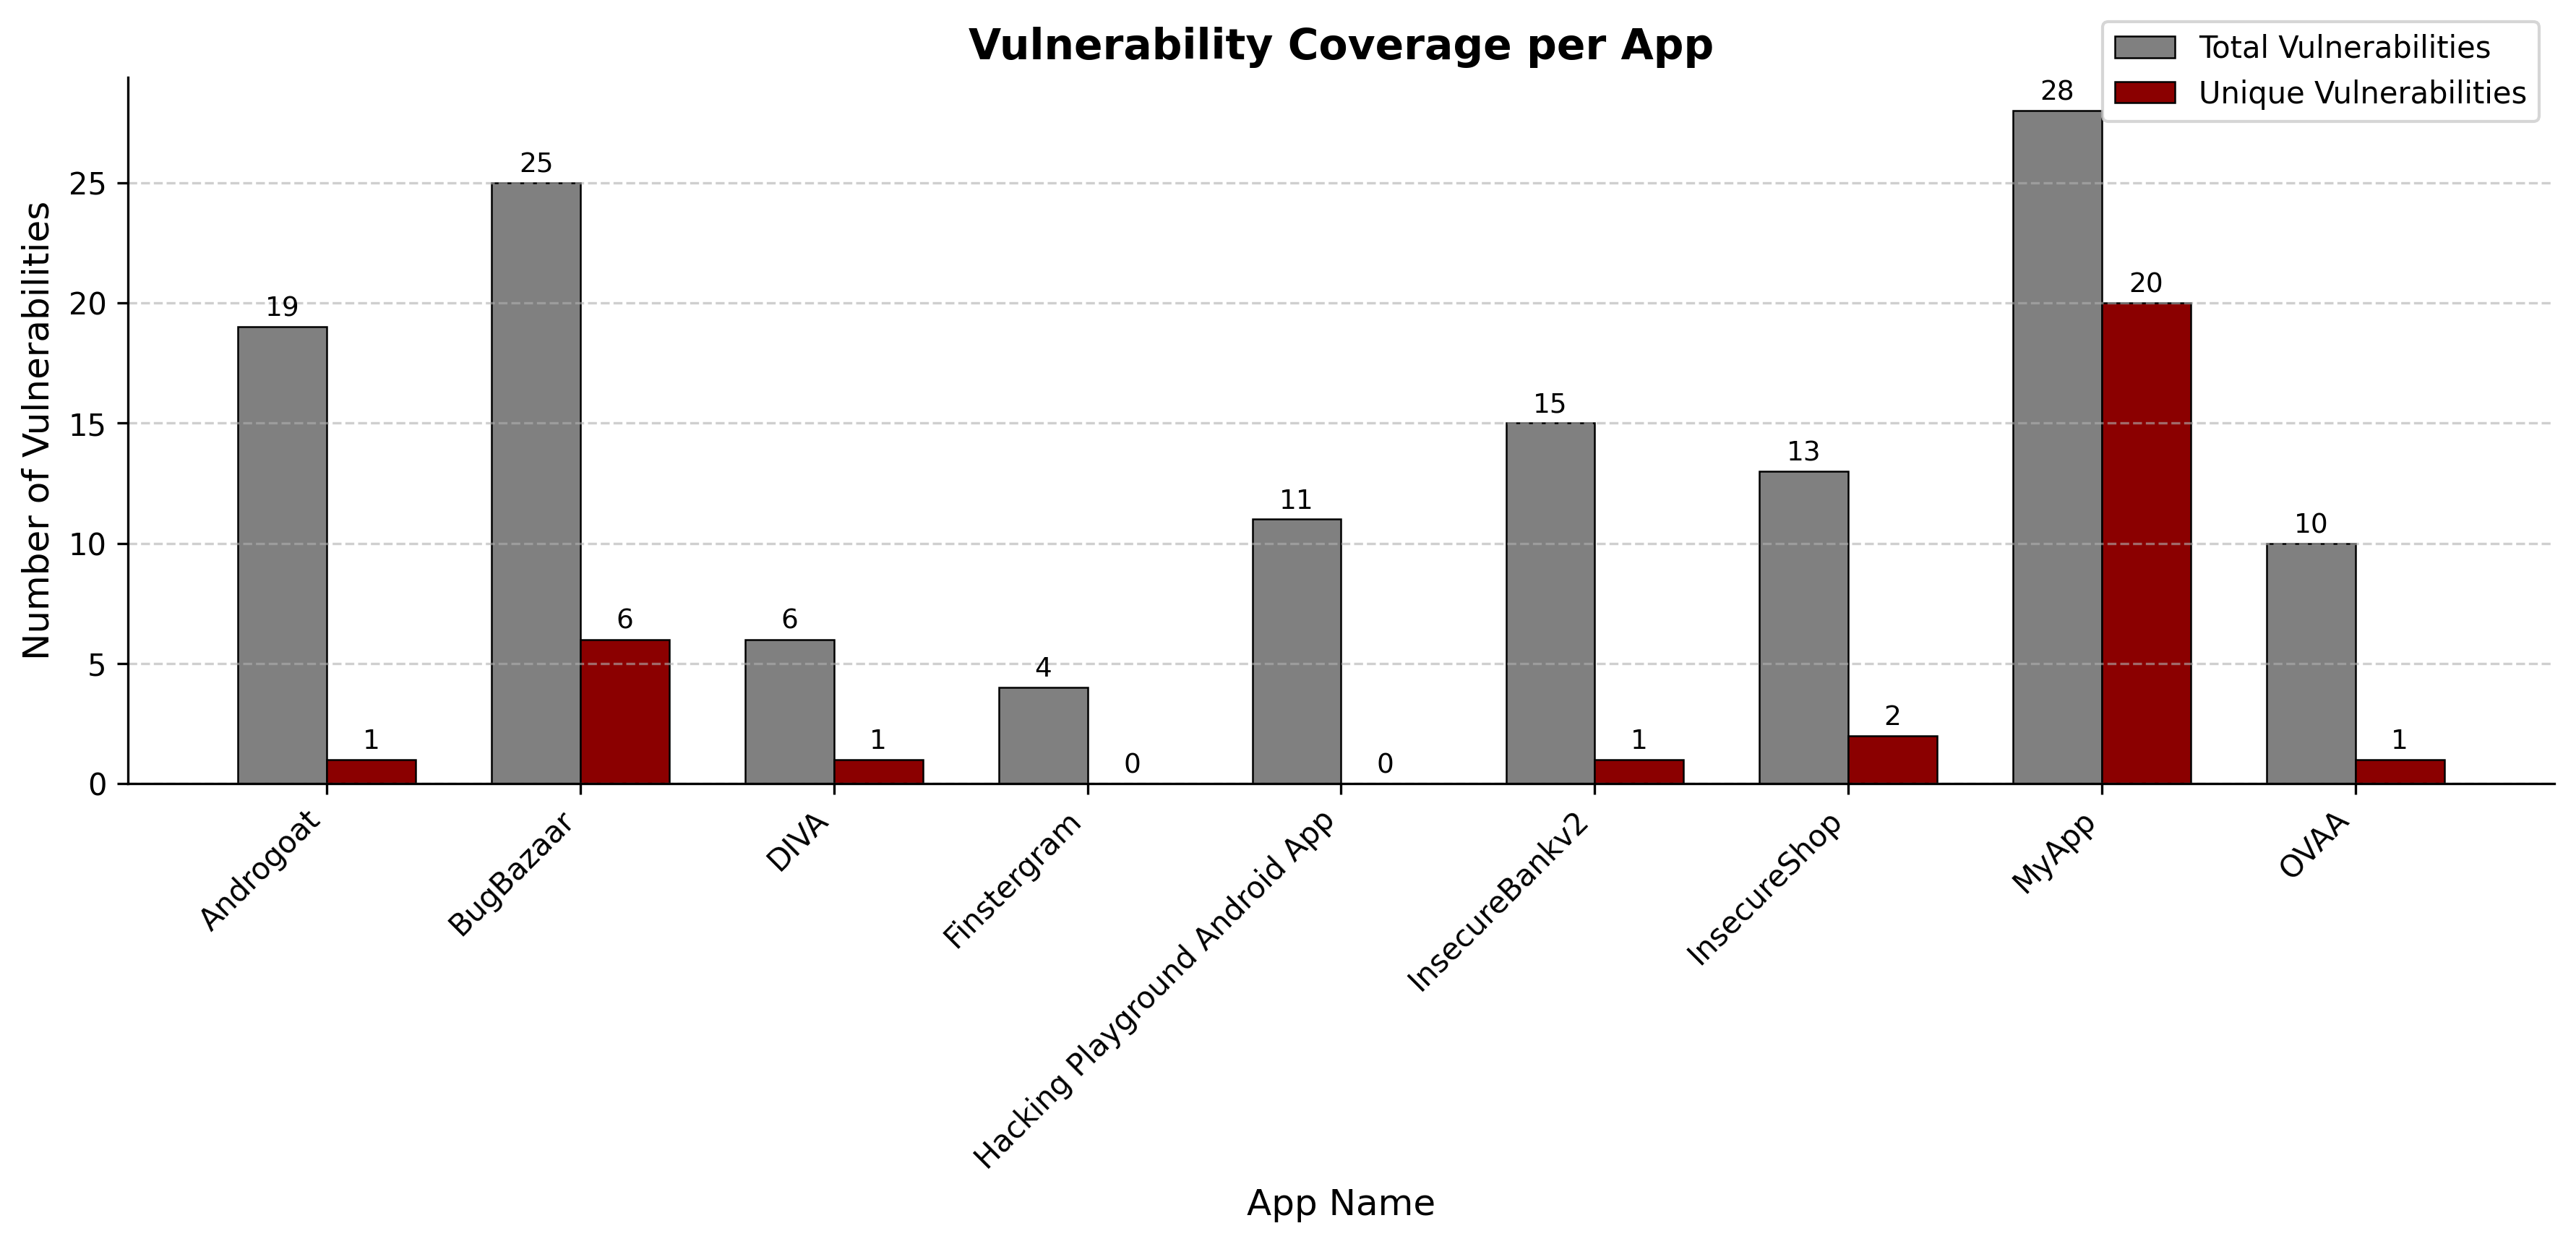
\includegraphics[width=1.0\textwidth]{dev_documents/BA_Thesis_Kronig/figures/results/total_vs_unique_with_own_app.png}
  \caption{ \todo{Add image caption} }
  \label{fig:}
\end{figure}


\begin{figure}[htbp]
  \centering
  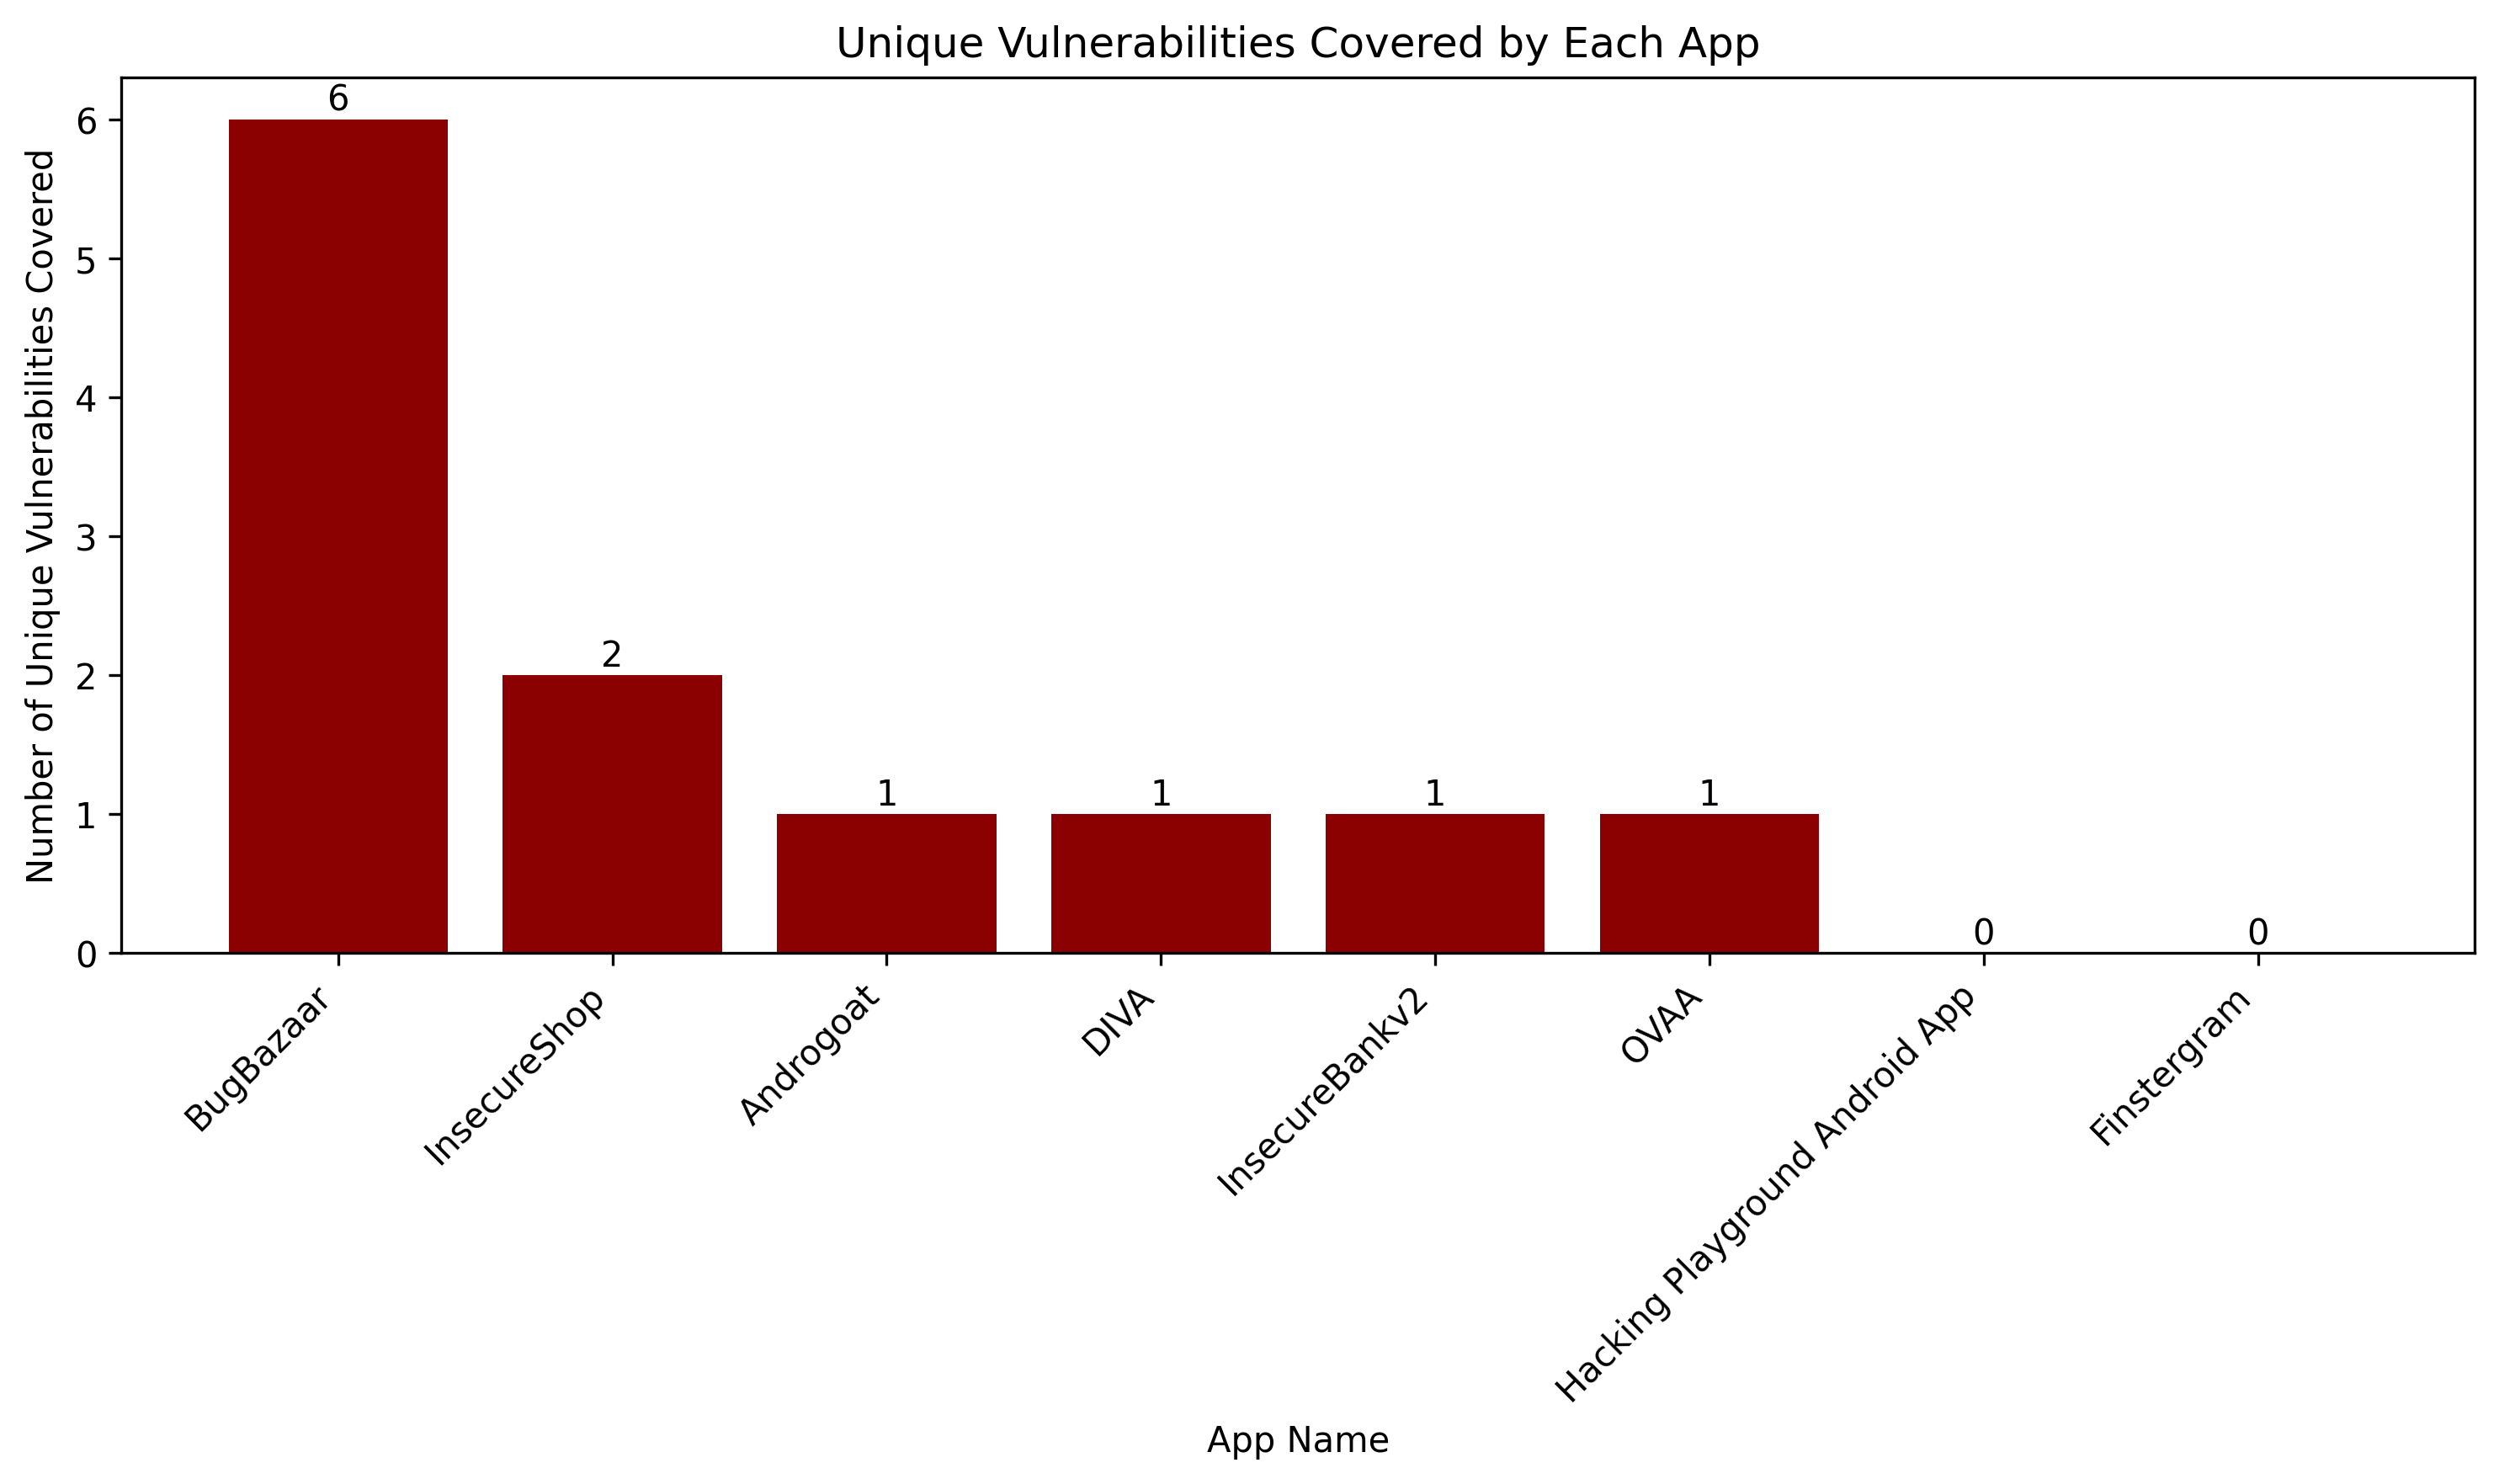
\includegraphics[width=1.0\textwidth]{dev_documents/BA_Thesis_Kronig/figures/results/unique_without_own_app.png}
  \caption{ \todo{Add image caption} }
  \label{fig:}
\end{figure}


\begin{figure}[htbp]
  \centering
  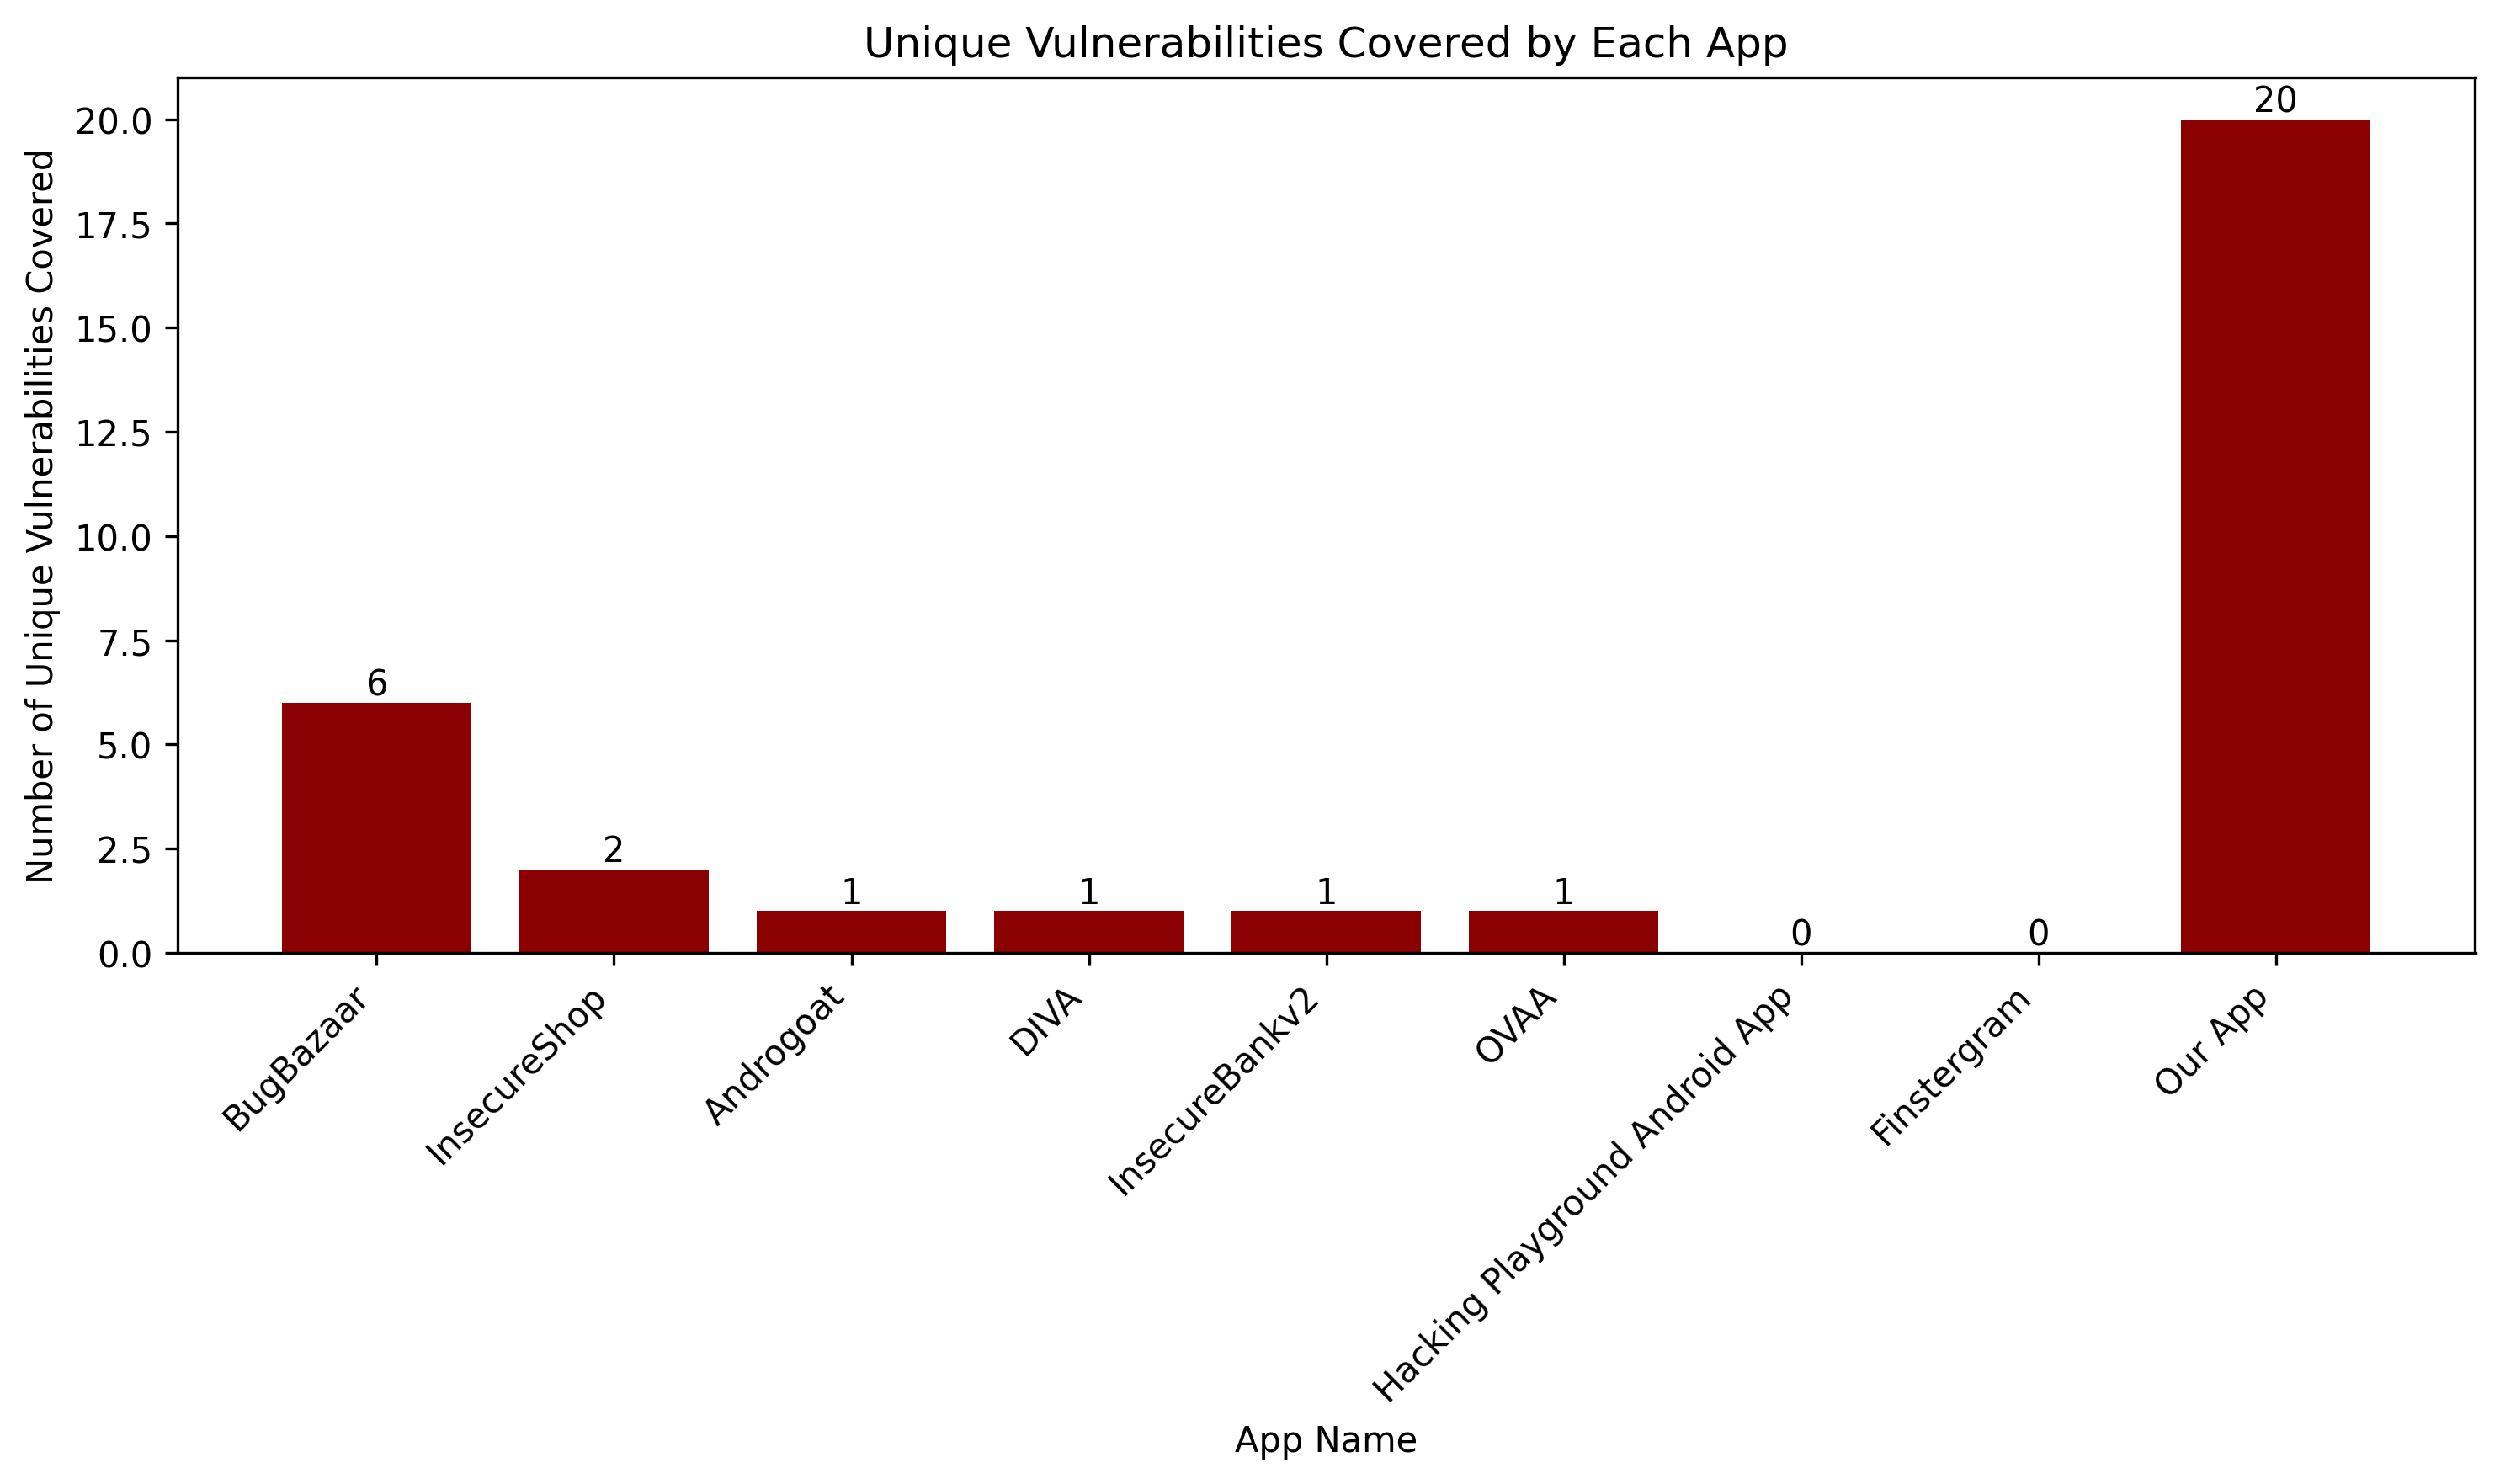
\includegraphics[width=1.0\textwidth]{dev_documents/BA_Thesis_Kronig/figures/results/unique_with_own_app.png}
  \caption{ \todo{Add image caption} }
  \label{fig:}
\end{figure}

\begin{figure}[htbp]
  \centering
  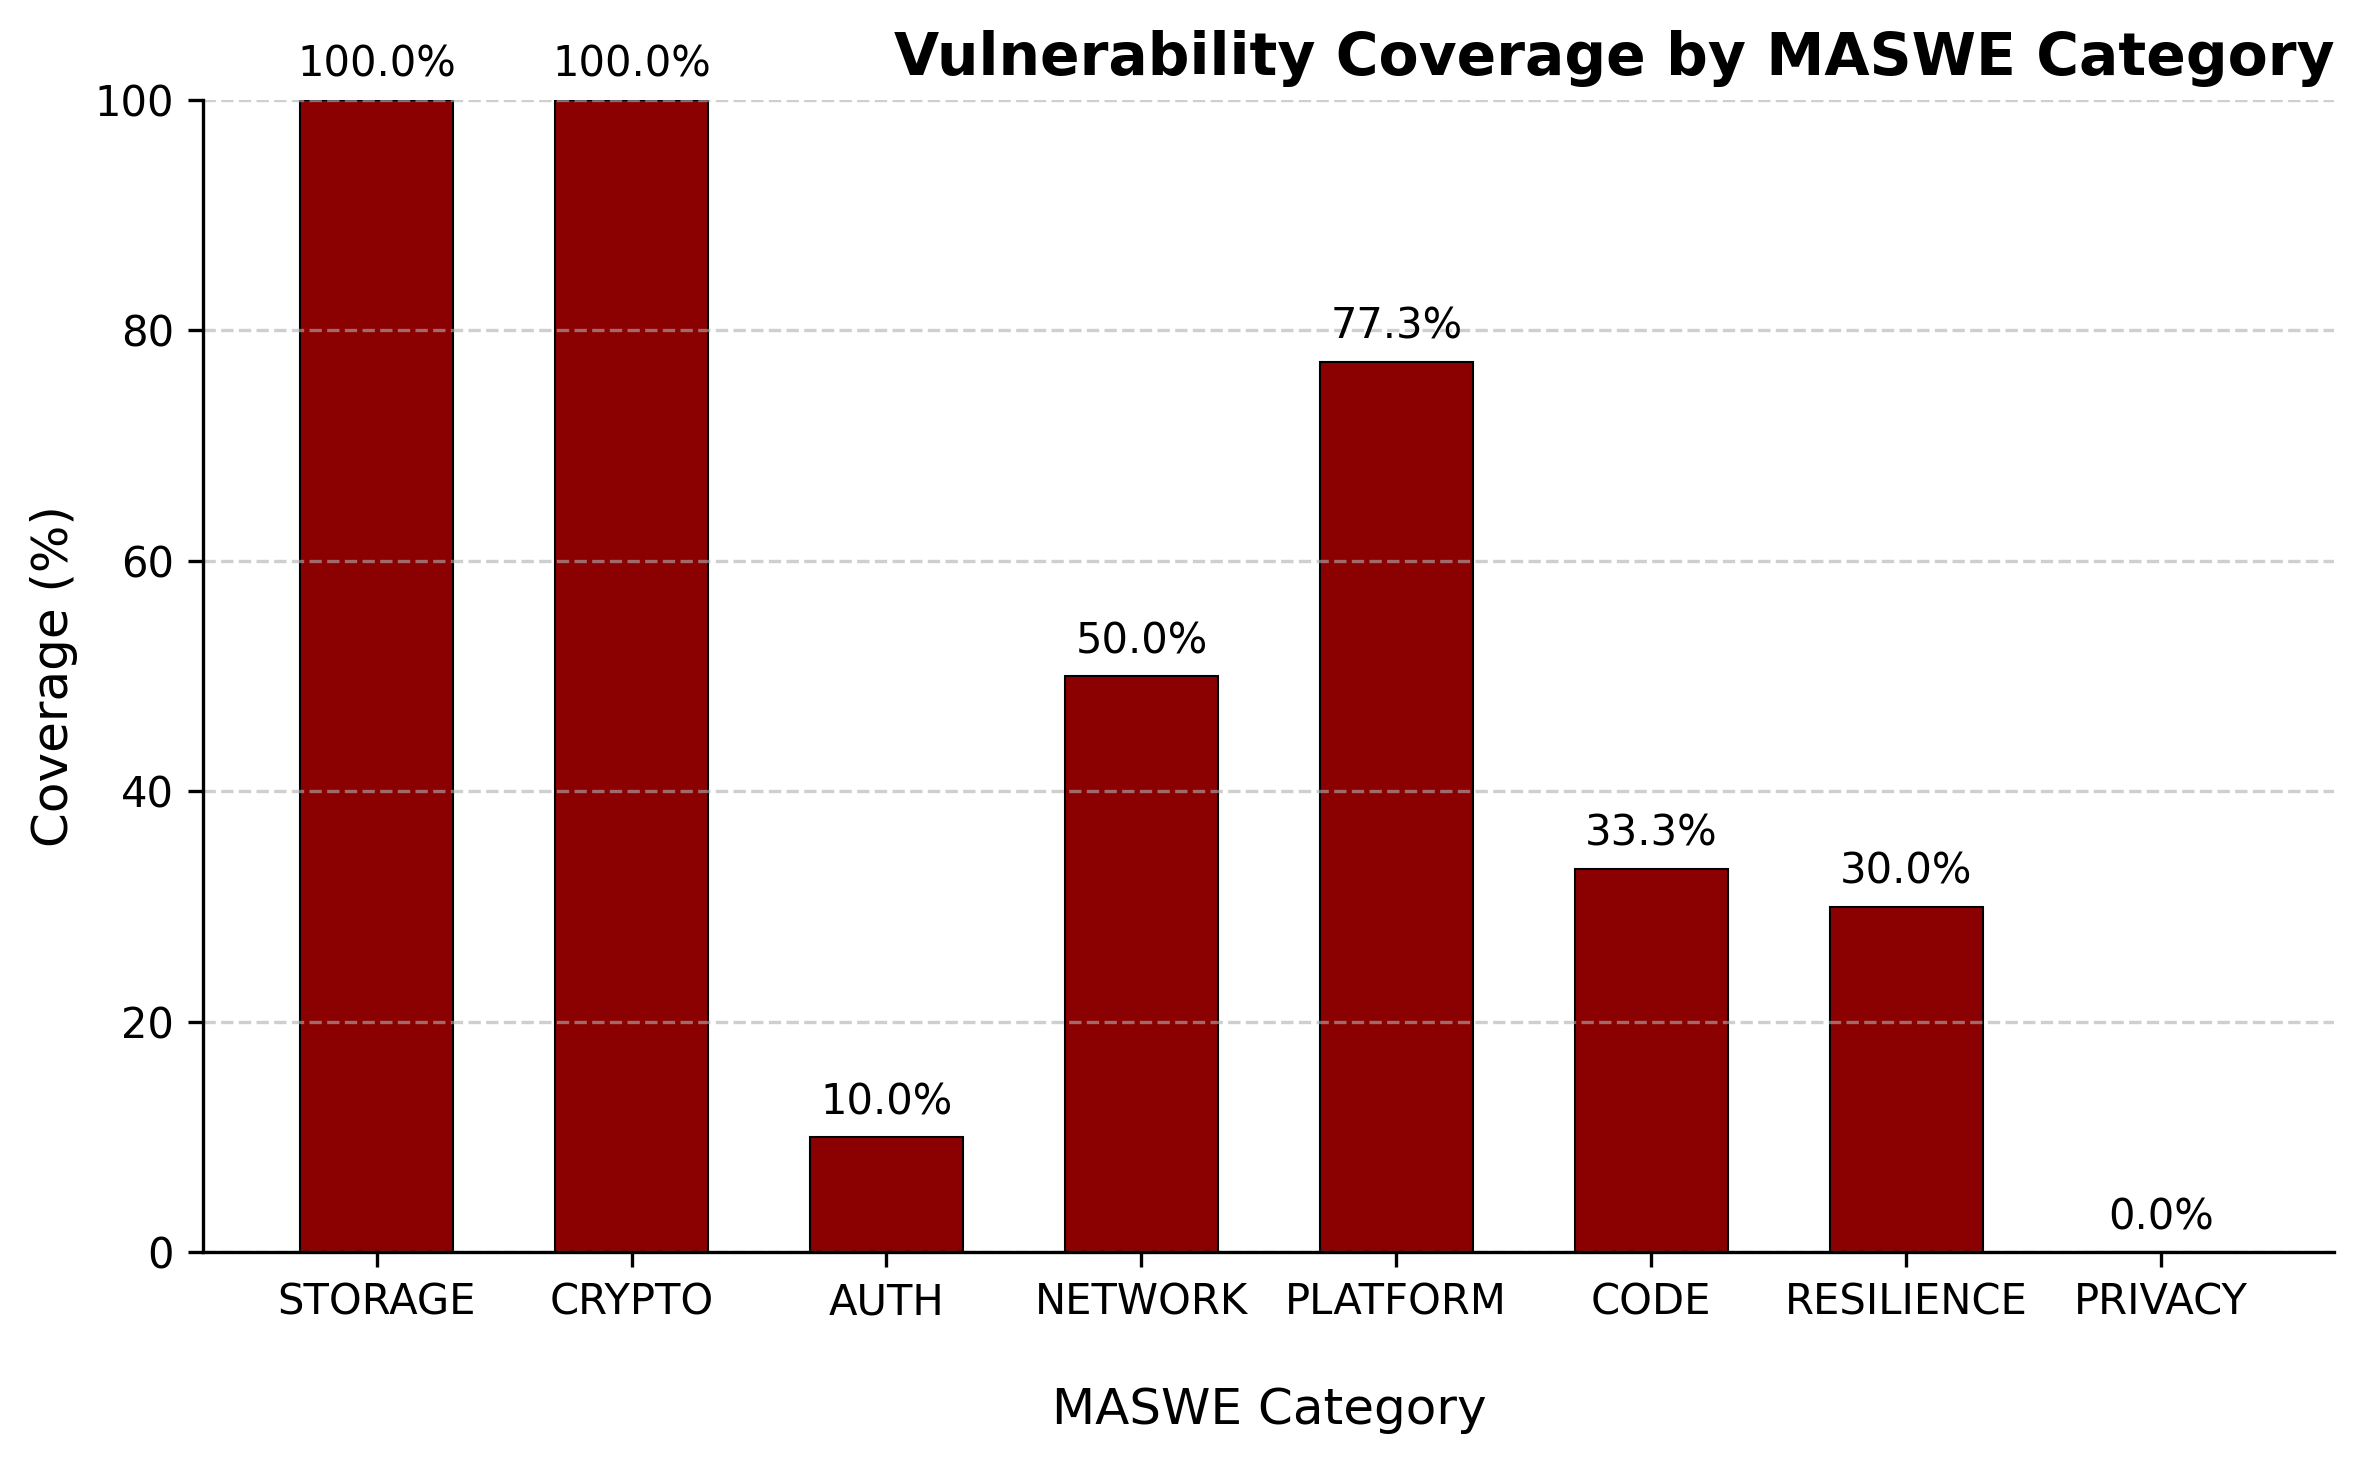
\includegraphics[width=1.0\textwidth]{dev_documents/BA_Thesis_Kronig/figures/results/vulnerability_coverage_percentage_with_own_app.png}
  \caption{ \todo{Add image caption} }
  \label{fig:}
\end{figure}


\section{Answers to Research Questions / Hypotheses}
